\documentclass[12pt,a4paper]{article}

\usepackage[utf8]{inputenc}
\usepackage[T1]{fontenc}
\usepackage{lmodern}
\usepackage{geometry}
\usepackage{graphicx}
\usepackage{booktabs}
\usepackage{longtable}
\usepackage{array}
\usepackage{float}
\usepackage{xcolor}
\usepackage{hyperref}
\usepackage{fancyhdr}
\usepackage{caption}
\usepackage{enumitem}
\usepackage{amsmath}

\geometry{left=1in,right=1in,top=1in,bottom=1in}
\newcolumntype{L}[1]{>{\raggedright\arraybackslash}p{#1}}
\hypersetup{
    colorlinks=true,
    linkcolor=blue,
    urlcolor=blue,
    citecolor=blue
}

\pagestyle{fancy}
\fancyhf{}
\lhead{Machine Learning Final Project}
\rhead{Scholarship Prediction}
\cfoot{\thepage}

\setlength{\parindent}{0pt}
\setlength{\parskip}{0.65em}
\setlength{\emergencystretch}{2em}
\sloppy
\setlist[itemize]{topsep=0.2em,itemsep=0.2em}
\setlist[enumerate]{topsep=0.2em,itemsep=0.2em}

\title{\textbf{Machine Learning Project Report}\\
\large Final Project: Scholarship Prediction System}
\author{Chau Pham Tuan Kiet - 523K0011\\Chau Thanh Vu - 523K0032\\Tran Anh Minh - 523K0017\\Course: Introduction to Machine Learning}
\date{April 29, 2026}

\begin{document}

\begin{titlepage}
    \centering
    \vspace*{1.2cm}
    {\Huge \textbf{Machine Learning Project Report}\par}
    \vspace{0.4cm}
    {\Large Final Project: Scholarship Prediction System\par}
    \vspace{1.5cm}
    \begin{tabular}{lp{0.68\linewidth}}
        Course: & Introduction to Machine Learning \\
        Project Type: & Final Project \\
        Dataset: & Synthetic Student Scholarship Dataset v2 \\
        Team Members: & Chau Pham Tuan Kiet - 523K0011\newline
        Chau Thanh Vu - 523K0032\newline
        Tran Anh Minh - 523K0017 \\
        Required Files: & report.pdf, notebook.ipynb, predictions.csv \\
        Recommended Files: & README.md, requirements.txt \\
    \end{tabular}
    \vfill
    \textbf{Implementation Note}\\
    All machine learning models in this project are implemented with Python and NumPy.
    The notebook does not use scikit-learn training APIs.
    \vfill
    {\large April 29, 2026\par}
\end{titlepage}

\tableofcontents
\clearpage

\section{Introduction}

The objective of this final project is to develop a complete machine learning pipeline for predicting scholarship eligibility. Each row in the dataset represents one student, and the model predicts whether that student receives a scholarship. This is a binary classification problem because the target variable has two possible values: label 1 for scholarship received and label 0 for scholarship not received.

This final version extends the midterm project. The midterm project established a basic pipeline with exploratory data analysis, preprocessing, model training, model evaluation, and error analysis. The final project keeps that same simple report structure, but it adds a more rigorous comparison of models, a meaningful improvement strategy, feature engineering, model interpretation, and a clearer final recommendation.

The goal is not only to obtain a high score on the development set. A strong final submission must also explain why each preprocessing and modeling decision was made. For that reason, this report emphasizes evidence from the data, reproducibility, avoidance of data leakage, and honest discussion of limitations.

\subsection{Project Scope}

The project scope is defined by the official final handout. The system must reconstruct a baseline based on the midterm project and then improve it in a meaningful way. At least three classical machine learning models must be trained and compared. The model set must include a linear model, a tree-based model, and another classical model.

The required evaluation metrics are accuracy, precision, recall, F1-score, and confusion matrix. ROC-AUC is also reported because prediction scores are available for the implemented models. The final report must include error analysis, model interpretation, and a final recommendation.

\subsection{Main Deliverables}

\begin{itemize}
    \item \texttt{report.pdf}: the final report compiled from this LaTeX source.
    \item \texttt{main.tex}: the LaTeX source file used to generate the report.
    \item \texttt{notebook.ipynb}: the reproducible implementation notebook.
    \item \texttt{predictions.csv}: prediction file with columns \texttt{id,label\_pred}.
    \item \texttt{README.md}: instructions for running the notebook locally or on Google Colab.
    \item \texttt{requirements.txt}: Python package requirements.
\end{itemize}

\subsection{Team Contribution Statement}

All team members contributed to the final project and reviewed the final notebook, report, and prediction file before submission. The work was divided as follows:

\begin{itemize}
    \item \textbf{Chau Pham Tuan Kiet - 523K0011}: prepared the project files for submission, checked data paths, verified the \texttt{predictions.csv} format, cleaned the notebook for reproducibility, and ran the final submission checks.
    \item \textbf{Chau Thanh Vu - 523K0032}: implemented the main preprocessing pipeline, feature engineering, scaling workflow, Logistic Regression and KNN models, and supported hyperparameter and threshold tuning.
    \item \textbf{Tran Anh Minh - 523K0017}: performed exploratory data analysis, implemented and reviewed the tree-based models, prepared the model comparison, error analysis, model interpretation, and polished the technical report.
\end{itemize}

The responsibilities were coordinated so that the workload remained balanced, while each member focused on the part most suitable for their role in the project.

\clearpage

\section{Dataset}

The dataset represents synthetic student records in a hypothetical country. Each row describes one student using academic and socio-economic attributes. The target is whether the student receives a scholarship.

The final training set contains 250 samples and 8 columns. The final development set contains 100 samples and 8 columns. The course already provides the train and development split, so the development set is used for evaluation and comparison after training.

\begin{table}[H]
\centering
\caption{Feature descriptions.}
\begin{tabular}{p{0.28\linewidth}p{0.62\linewidth}}
\toprule
\textbf{Feature Name} & \textbf{Brief Description} \\
\midrule
\texttt{id} & Unique row identifier. It is preserved for output but removed from model features. \\
\texttt{gpa} & Grade Point Average on a 2.0 to 4.0 scale. \\
\texttt{attendance\_rate} & Proportion of attended classes from 0 to 1. \\
\texttt{study\_hours\_per\_week} & Average weekly self-study hours. \\
\texttt{exam\_score} & Final exam score. \\
\texttt{household\_income} & Approximate synthetic household monthly income. \\
\texttt{part\_time\_job\_hours} & Weekly part-time work hours, added in the final v2 dataset. \\
\texttt{label} & Target variable: 1 means scholarship, 0 means no scholarship. \\
\bottomrule
\end{tabular}
\end{table}

The \texttt{id} column is kept for writing predictions, but it is removed before training. The reason is simple: an identifier is not a real student characteristic. If the model learns patterns from id values, the result would be misleading and unlikely to generalize.

\clearpage

\subsection{Difference from the Midterm Dataset}

The final dataset extends the midterm dataset. The most important difference is the addition of \texttt{part\_time\_job\_hours}. This feature is meaningful because part-time work may affect the balance between study time and other responsibilities.

\begin{table}[H]
\centering
\caption{Midterm and final dataset comparison.}
\begin{tabular}{lll}
\toprule
\textbf{Aspect} & \textbf{Midterm} & \textbf{Final} \\
\midrule
Training samples & 200 & 250 \\
Development samples & 80 & 100 \\
Base feature count & 5 & 6 \\
New feature & None & \texttt{part\_time\_job\_hours} \\
Train positive rate & about 39\% & 40\% \\
\bottomrule
\end{tabular}
\end{table}

The hidden test file is read from \texttt{hidden\_test\_data.csv}. If the hidden test schema does not include \texttt{part\_time\_job\_hours}, the notebook fills the missing final-only feature with the median value from the final training set.

\clearpage

\section{Exploratory Data Analysis}

Exploratory Data Analysis is used to understand the structure and behavior of the dataset before modeling. The purpose is not to create random charts, but to identify information that supports later preprocessing and model-selection decisions.

The final training set contains 150 non-scholarship students and 100 scholarship students. The final development set contains 60 non-scholarship students and 40 scholarship students. This indicates a moderate class imbalance. The imbalance is not extreme, but it is enough that precision, recall, and F1-score are more informative than accuracy alone.

\begin{figure}[H]
\centering
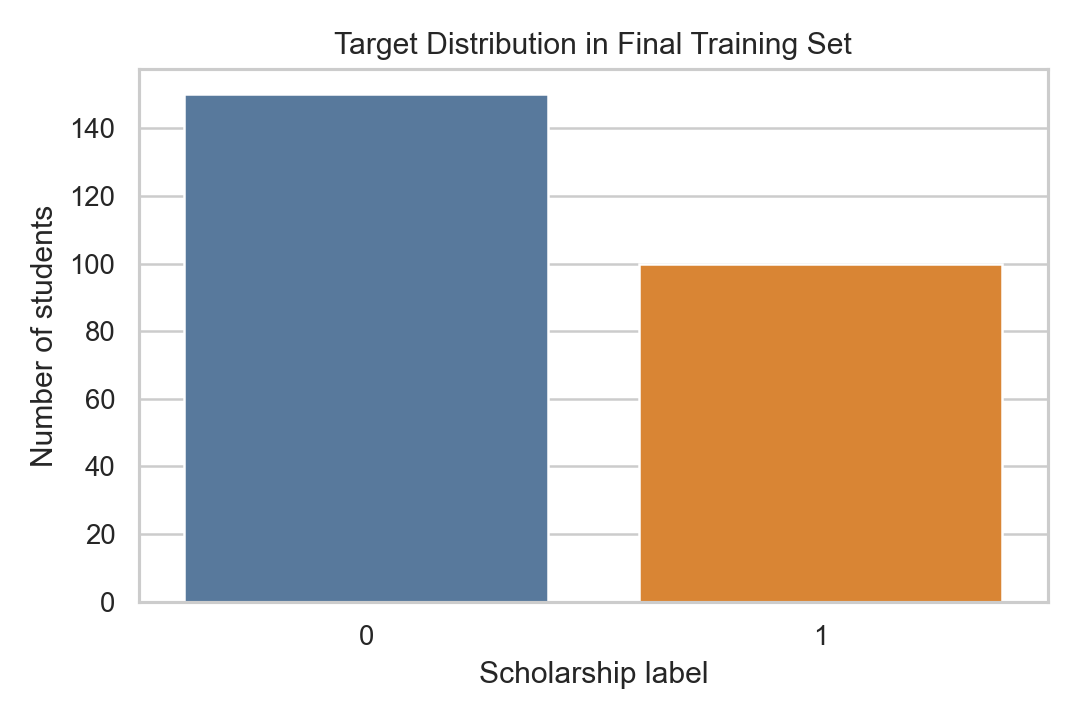
\includegraphics[width=0.76\linewidth]{figures/target_distribution.png}
\caption{Target distribution in the final training set.}
\end{figure}

The target distribution is important for metric selection. If a model predicts mostly the majority class, accuracy alone could look acceptable while recall for scholarship recipients becomes poor. Therefore, this report treats F1-score and recall as important metrics.

\clearpage

\subsection{Descriptive Statistics}

\begin{table}[H]
\centering
\caption{Descriptive statistics for final training features.}
\begin{tabular}{lrrrrrr}
\toprule
 & \textbf{gpa} & \textbf{attendance} & \textbf{study hrs} & \textbf{exam} & \textbf{income} & \textbf{job hrs} \\
\midrule
count & 250.000 & 250.000 & 250.000 & 250.000 & 250.000 & 250.000 \\
mean & 3.005 & 0.804 & 21.984 & 71.568 & 1394.744 & 12.500 \\
std & 0.598 & 0.117 & 9.647 & 16.087 & 656.450 & 7.433 \\
min & 2.000 & 0.600 & 5.000 & 45.000 & 205.000 & 0.000 \\
25\% & 2.445 & 0.710 & 14.000 & 57.000 & 873.000 & 6.000 \\
50\% & 3.015 & 0.805 & 22.000 & 71.500 & 1436.500 & 13.000 \\
75\% & 3.500 & 0.910 & 30.000 & 85.000 & 1957.250 & 19.000 \\
max & 3.990 & 1.000 & 39.000 & 99.000 & 2497.000 & 24.000 \\
\bottomrule
\end{tabular}
\end{table}

The numeric ranges differ substantially across features. GPA has a small range, while household income has values in the hundreds or thousands. This difference supports the decision to standardize features before training models such as Logistic Regression and KNN.

\clearpage

\subsection{Correlation Analysis}

\begin{figure}[H]
\centering
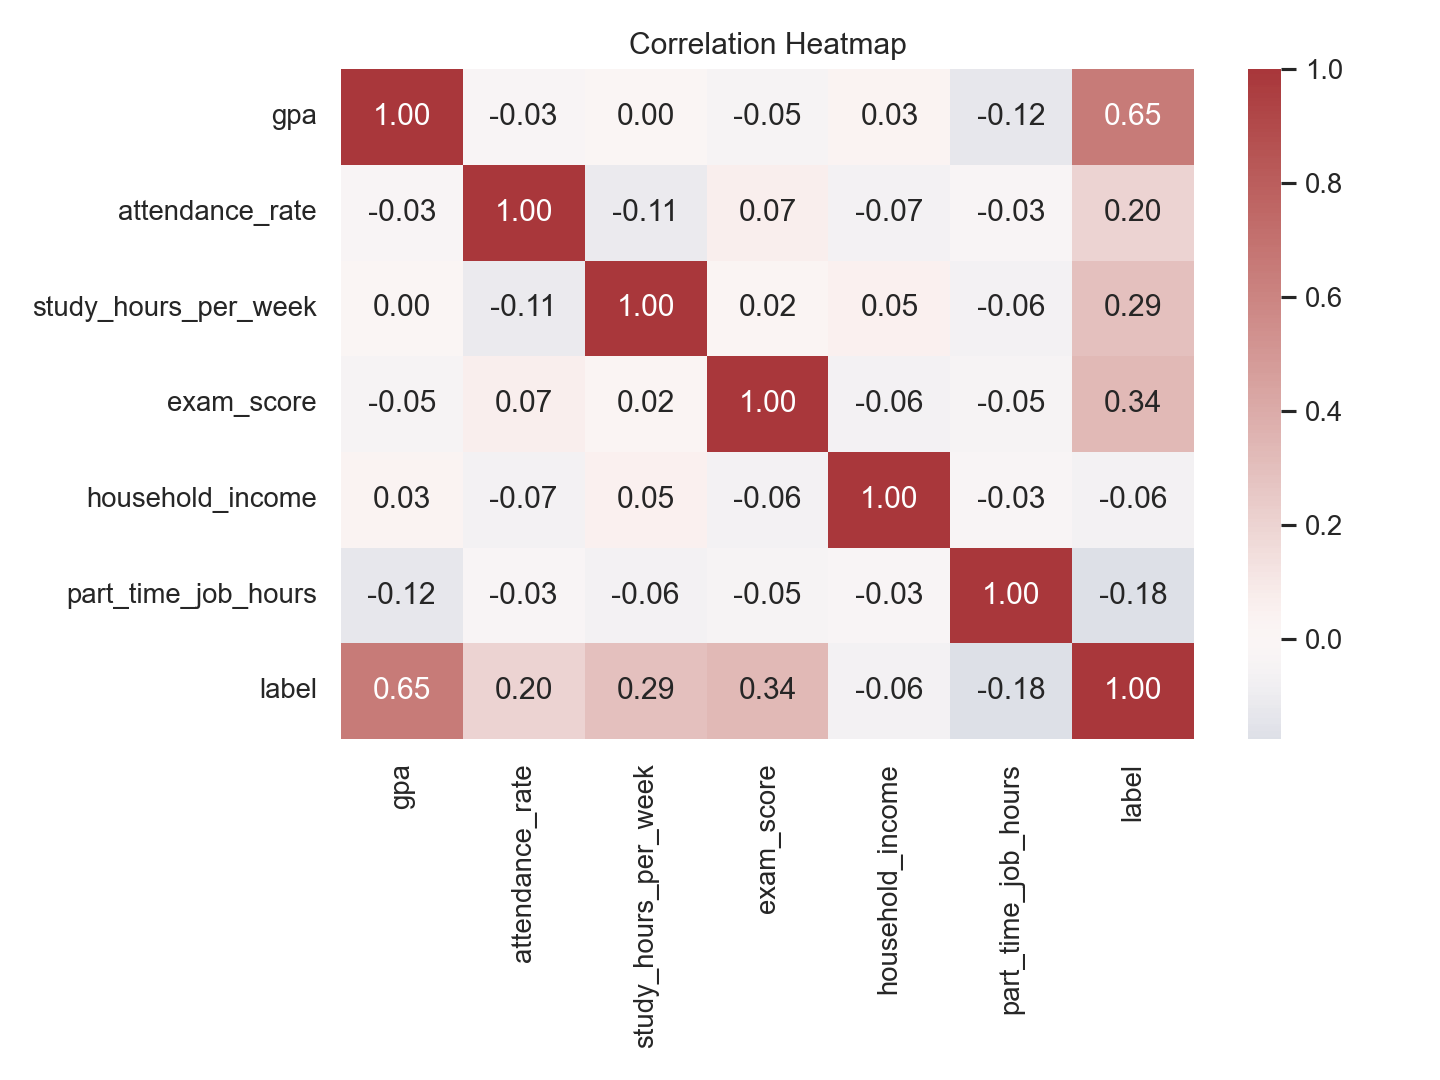
\includegraphics[width=0.86\linewidth]{figures/correlation_heatmap.png}
\caption{Correlation heatmap for final training features.}
\end{figure}

Correlation is useful for initial exploration, but it should not be interpreted as causation. A feature can be correlated with scholarship status without directly causing that outcome. The correlation heatmap is used as guidance for modeling and interpretation, not as final proof.

Academic variables such as GPA and exam score are expected to be relevant to scholarship status. Socio-economic variables and part-time work variables may also be useful, but their effects are more subtle and should be evaluated through model performance and feature importance rather than visual inspection alone.

\clearpage

\subsection{GPA and Scholarship Status}

\begin{figure}[H]
\centering
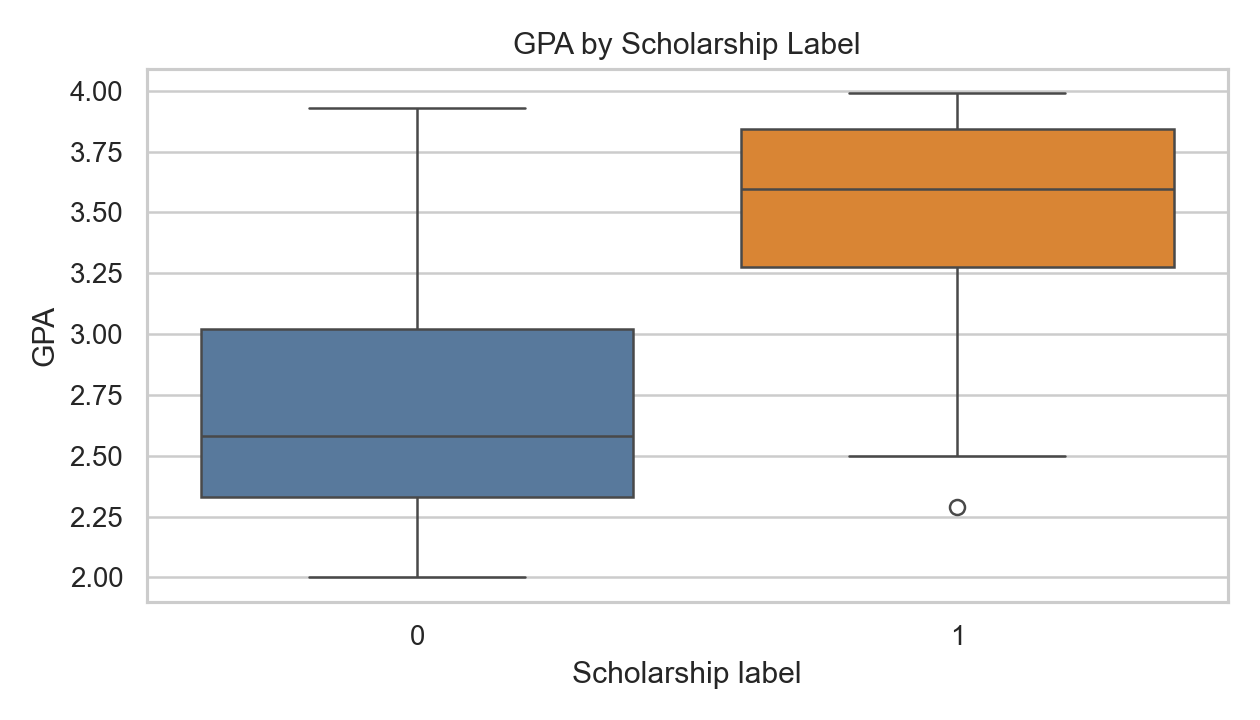
\includegraphics[width=0.78\linewidth]{figures/gpa_by_label.png}
\caption{GPA distribution by scholarship label.}
\end{figure}

The GPA distribution by class helps verify whether academic performance is related to the target variable. If scholarship recipients tend to have higher GPA values, this supports the intuition that academic merit is an important signal for the prediction problem.

This observation is consistent with the problem context, but the model should not rely on one feature only. Students may have different combinations of GPA, exam score, study hours, income, and part-time work hours. A full model comparison is therefore still necessary.

\clearpage

\subsection{Part-Time Job Hours}

\begin{figure}[H]
\centering
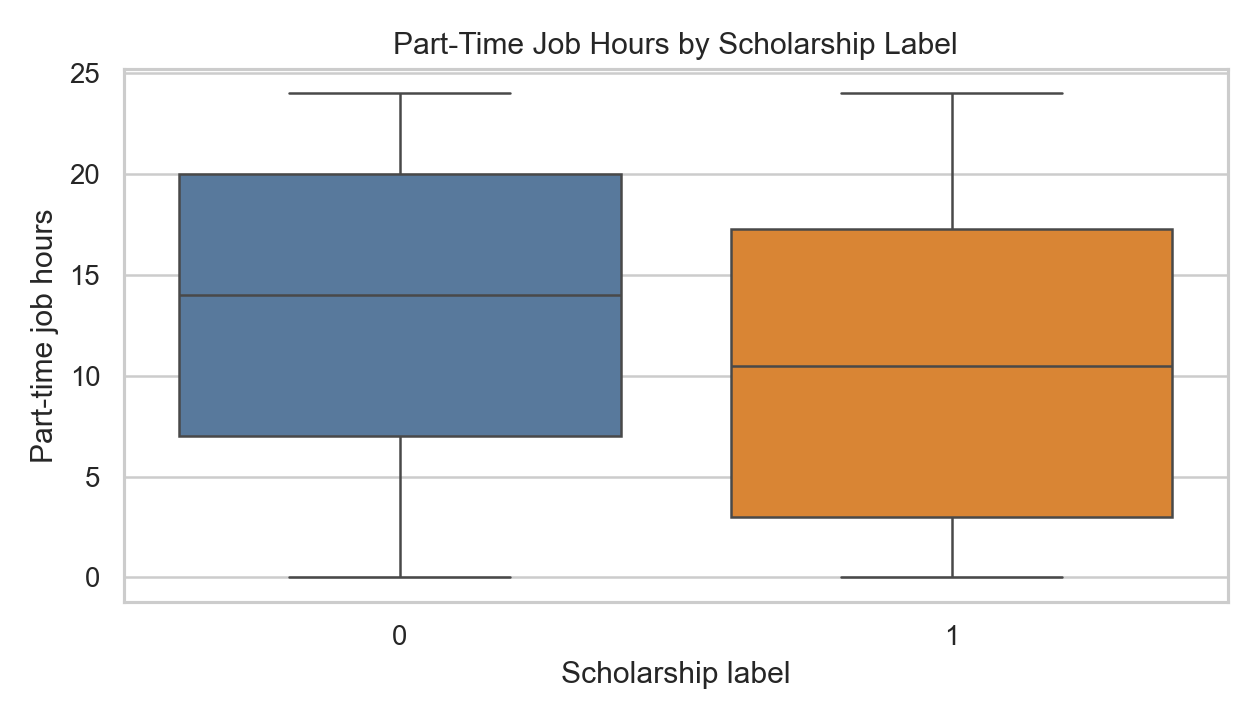
\includegraphics[width=0.78\linewidth]{figures/part_time_by_label.png}
\caption{Part-time job hours by scholarship label.}
\end{figure}

Part-time job hours are especially important because they were not present in the midterm dataset. This feature may capture outside work burden or time constraints. Even when a single feature is not strongly separated by label, it can still help in combination with study hours, exam score, and GPA.

Because this feature is new in the final dataset, it is included in the final feature set and also used to construct one engineered feature: \texttt{work\_study\_balance}.

\clearpage

\section{Data Preprocessing}

The preprocessing workflow follows the same basic structure as the midterm report, but it is implemented fully manually. First, required columns are validated. Second, the \texttt{id} column is removed from the feature matrix. Third, missing values are checked. Fourth, features are standardized using a scaler fitted only on training data.

\begin{table}[H]
\centering
\caption{Preprocessing decisions.}
\small
\begin{tabular}{L{0.22\linewidth}L{0.28\linewidth}L{0.38\linewidth}}
\toprule
\textbf{Step} & \textbf{Decision} & \textbf{Justification} \\
\midrule
Missing values & No train/dev imputation required & Both final train and dev have zero missing values. \\
Categorical encoding & Not required & All provided final features are numeric. \\
ID handling & Drop \texttt{id} from features & Identifier values should not drive prediction. \\
Scaling & Standardize numeric features & Needed for Logistic Regression and KNN. \\
Leakage control & Fit scaler on train only & Development and hidden data must remain unseen during fitting. \\
\bottomrule
\end{tabular}
\end{table}

The most important methodological point is leakage prevention. The scaler computes means and standard deviations from the training set only. The same stored values are then reused to transform development and hidden data.

\clearpage

\subsection{Feature Engineering}

The final project includes feature engineering as one meaningful improvement over the midterm baseline. These features are simple enough to explain and are created only from input variables.

\begin{table}[H]
\centering
\caption{Engineered features.}
\small
\begin{tabular}{L{0.27\linewidth}L{0.31\linewidth}L{0.30\linewidth}}
\toprule
\textbf{New Feature} & \textbf{Formula} & \textbf{Reason} \\
\midrule
\texttt{academic\_strength} & \texttt{gpa * exam\_score} & Combines long-term and exam performance. \\
\texttt{study\_efficiency} & \texttt{exam\_score / (study\_hours + 1)} & Measures exam score relative to study time. \\
\texttt{income\_per\_study\_hour} & \texttt{income / (study\_hours + 1)} & Combines economic context and study effort. \\
\texttt{work\_study\_balance} & \texttt{study\_hours - job\_hours} & Captures balance between studying and working. \\
\bottomrule
\end{tabular}
\end{table}

These engineered features are created only from input features, not from label values. Therefore, they do not leak the answer into the model. They are included as the main final improvement over the midterm-style baseline.

\clearpage

\section{Models}

The final project compares four classical machine learning models. All models are trained manually using NumPy operations rather than scikit-learn training APIs. This satisfies the implementation constraint while keeping the workflow understandable.

\begin{table}[H]
\centering
\caption{Models used in the final project.}
\small
\begin{tabular}{L{0.25\linewidth}L{0.30\linewidth}L{0.35\linewidth}}
\toprule
\textbf{Model} & \textbf{Role} & \textbf{Why It Was Chosen} \\
\midrule
Logistic Regression & Required linear model and final recommendation & Interpretable, stable, and strong on this data. \\
Decision Tree & Tree-based baseline & Easy to explain using split rules. \\
Random Forest & Tree-based ensemble & More stable than a single decision tree. \\
KNN & Additional classical model & Simple distance-based model that is easy to implement manually. \\
\bottomrule
\end{tabular}
\end{table}

The models represent different assumptions. Logistic Regression assumes a mostly linear relationship after scaling. Decision Tree and Random Forest can capture non-linear splits. KNN predicts based on local similarity in feature space.

\clearpage

\subsection{Logistic Regression}

Logistic Regression computes a weighted sum of the input features and converts it into a probability using the sigmoid function:

\[
    \hat{p} = \frac{1}{1 + e^{-(w^Tx + b)}}
\]

If the probability is greater than the selected threshold, the model predicts scholarship. The weights are learned with gradient descent.

This model is the easiest to explain academically because each coefficient has a direction. A positive coefficient increases the predicted probability of scholarship, while a negative coefficient decreases it. Since features are standardized, coefficient magnitudes are more comparable.

For the final model, the selected Logistic Regression settings are:

\begin{itemize}
    \item Learning rate: 0.03
    \item Number of iterations: 5000
    \item L2 regularization: 0.0
    \item Decision threshold: 0.55
\end{itemize}

\clearpage

\subsection{Decision Tree}

The Decision Tree uses Gini impurity to select feature thresholds that separate the two classes. At each node, the algorithm searches for a split that reduces impurity. The implementation uses maximum depth and minimum samples per split to reduce overfitting.

The Gini impurity for a binary node is:

\[
    Gini = 1 - p_1^2 - p_0^2
\]

where \(p_1\) is the proportion of scholarship students in the node and \(p_0\) is the proportion of non-scholarship students.

The main strength of the Decision Tree is interpretability. Its predictions can be described as if-then rules. The main weakness is that a single tree can overfit small datasets.

\clearpage

\subsection{Random Forest}

Random Forest trains multiple decision trees on bootstrap samples and random subsets of features. Predictions are averaged as probabilities. This usually improves stability and reduces the variance of a single tree.

The Random Forest implementation in the notebook uses the following ideas:

\begin{itemize}
    \item Bootstrap sampling of training examples.
    \item Random feature subsets at each tree.
    \item Multiple decision trees with controlled depth.
    \item Averaging of predicted probabilities.
\end{itemize}

Random Forest is included because it satisfies the tree-based model requirement and provides a useful comparison against both the simple Decision Tree and the linear model.

\clearpage

\subsection{KNN}

KNN predicts a new example by looking at the labels of the nearest training examples. Because it relies on distance, scaling is essential. In this project, weighted KNN is also tested so that closer neighbors can contribute more strongly than farther neighbors.

The KNN prediction process is simple:

\begin{enumerate}
    \item Standardize the new example using the training scaler.
    \item Compute distances from the new example to training examples.
    \item Select the \(k\) nearest examples.
    \item Average their labels, optionally with distance-based weights.
    \item Convert the average score to class 0 or 1.
\end{enumerate}

KNN is included as the additional classical model because it is simple, transparent, and fully implementable without external machine learning libraries.

\clearpage

\section{Improvement Strategy}

The final project must include at least one meaningful improvement over the midterm baseline. This submission includes several improvements, but the main improvement is the combination of final v2 features, engineered features, controlled hyperparameter tuning, and threshold selection.

\begin{table}[H]
\centering
\caption{Final improvements over the midterm-style baseline.}
\small
\begin{tabular}{L{0.24\linewidth}L{0.36\linewidth}L{0.30\linewidth}}
\toprule
\textbf{Improvement} & \textbf{Description} & \textbf{Evidence Used} \\
\midrule
Final v2 feature & Use \texttt{part\_time\_job\_hours} & Included in EDA and final modeling. \\
Feature engineering & Create four additional features & Included in improved model feature matrix. \\
Hyperparameter tuning & Small controlled grid per model & Internal validation F1-score. \\
Threshold tuning & Tune Logistic Regression threshold & Improves final F1/recall balance. \\
Interpretability & Coefficients and permutation importance & Explains model behavior. \\
\bottomrule
\end{tabular}
\end{table}

The tuning process uses an internal stratified validation split from the training data. This avoids tuning every decision directly on the final development set. After selecting settings, models are retrained on the full final training set and evaluated on the final development set.

\clearpage

\section{Experimental Results}

The experiments compare a midterm-style baseline and the improved final models. The baseline uses Logistic Regression with the original midterm feature set. The final models use the final feature set with engineered features and tuned hyperparameters.

\subsection{Baseline Result}

\begin{table}[H]
\centering
\caption{Midterm-style baseline result on final development data.}
\small
\begin{tabular}{lrrrrr}
\toprule
\textbf{Model} & \textbf{Accuracy} & \textbf{Precision} & \textbf{Recall} & \textbf{F1} & \textbf{ROC-AUC} \\
\midrule
Baseline Logistic Regression & 0.9000 & 1.0000 & 0.7500 & 0.8571 & 0.9963 \\
\bottomrule
\end{tabular}
\end{table}

The baseline provides a simple reference point. It is intentionally close to the midterm pipeline so that the final improvements can be judged against a clear starting point.

\clearpage

\subsection{Final Model Comparison}

\begin{table}[H]
\centering
\caption{Final model comparison on the development set.}
\begin{tabular}{lrrrrrrr}
\toprule
\textbf{Model} & \textbf{Acc.} & \textbf{Prec.} & \textbf{Rec.} & \textbf{F1} & \textbf{ROC-AUC} & \textbf{FP} & \textbf{FN} \\
\midrule
Logistic Regression & 0.9200 & 1.0000 & 0.8000 & 0.8889 & 0.9963 & 0 & 8 \\
KNN & 0.9200 & 1.0000 & 0.8000 & 0.8889 & 0.9933 & 0 & 8 \\
Random Forest & 0.8900 & 0.9394 & 0.7750 & 0.8493 & 0.9458 & 2 & 9 \\
Decision Tree & 0.7900 & 0.7714 & 0.6750 & 0.7200 & 0.7613 & 8 & 13 \\
\bottomrule
\end{tabular}
\end{table}

Logistic Regression and KNN achieved the same accuracy, precision, recall, and F1-score. Logistic Regression is selected because it has a slightly higher ROC-AUC and is easier to explain through coefficients.

\begin{figure}[H]
\centering
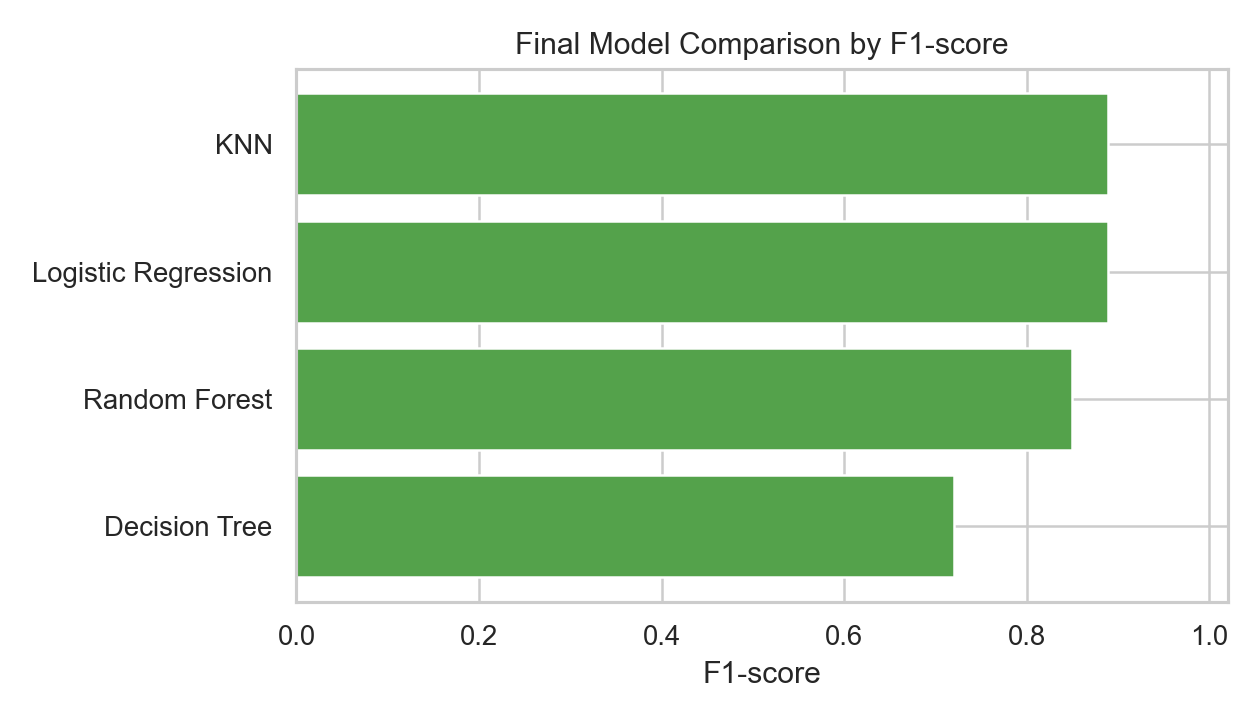
\includegraphics[width=0.80\linewidth]{figures/model_comparison_f1.png}
\caption{Final model comparison by F1-score.}
\end{figure}

\clearpage

\subsection{Confusion Matrix}

\begin{figure}[H]
\centering
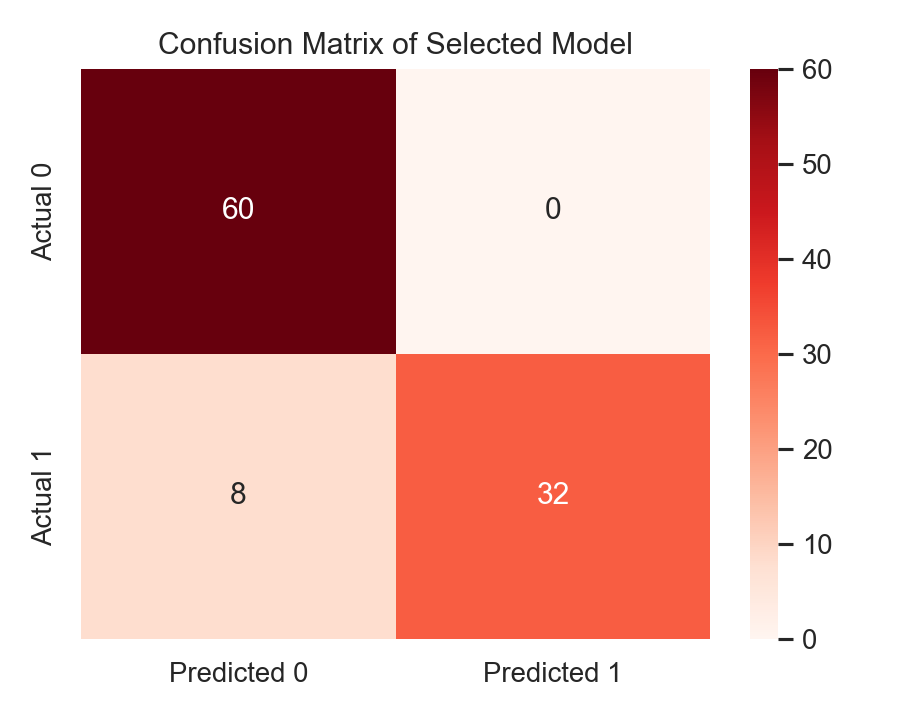
\includegraphics[width=0.72\linewidth]{figures/selected_confusion_matrix.png}
\caption{Confusion matrix for the selected Logistic Regression model.}
\end{figure}

The selected model produced 32 true positives, 60 true negatives, 0 false positives, and 8 false negatives. The model made no false positive errors on the development set, but it did miss some scholarship students. This explains why recall is lower than precision.

\clearpage

\section{Error Analysis}

Error analysis examines the actual cases that the model predicted incorrectly. This is important because metrics alone do not explain why a model fails.

\begin{table}[H]
\centering
\caption{Representative development-set errors.}
\begin{tabular}{rrrrrrr}
\toprule
\textbf{id} & \textbf{label} & \textbf{pred} & \textbf{score} & \textbf{gpa} & \textbf{exam} & \textbf{job hrs} \\
\midrule
5 & 1 & 0 & 0.4647 & 3.55 & 59 & 21 \\
6 & 1 & 0 & 0.2492 & 2.75 & 68 & 20 \\
8 & 1 & 0 & 0.2113 & 2.29 & 75 & 10 \\
10 & 1 & 0 & 0.5053 & 3.03 & 85 & 13 \\
15 & 1 & 0 & 0.3200 & 2.67 & 67 & 8 \\
24 & 1 & 0 & 0.3978 & 2.76 & 79 & 16 \\
68 & 1 & 0 & 0.3135 & 2.61 & 72 & 6 \\
86 & 1 & 0 & 0.4807 & 3.44 & 54 & 19 \\
\bottomrule
\end{tabular}
\end{table}

The errors are false negatives: students who received scholarships but were predicted as non-scholarship cases. This suggests that the selected threshold and linear boundary are conservative. The model avoids false positives, but at the cost of missing some positive cases.

\clearpage

\begin{figure}[H]
\centering
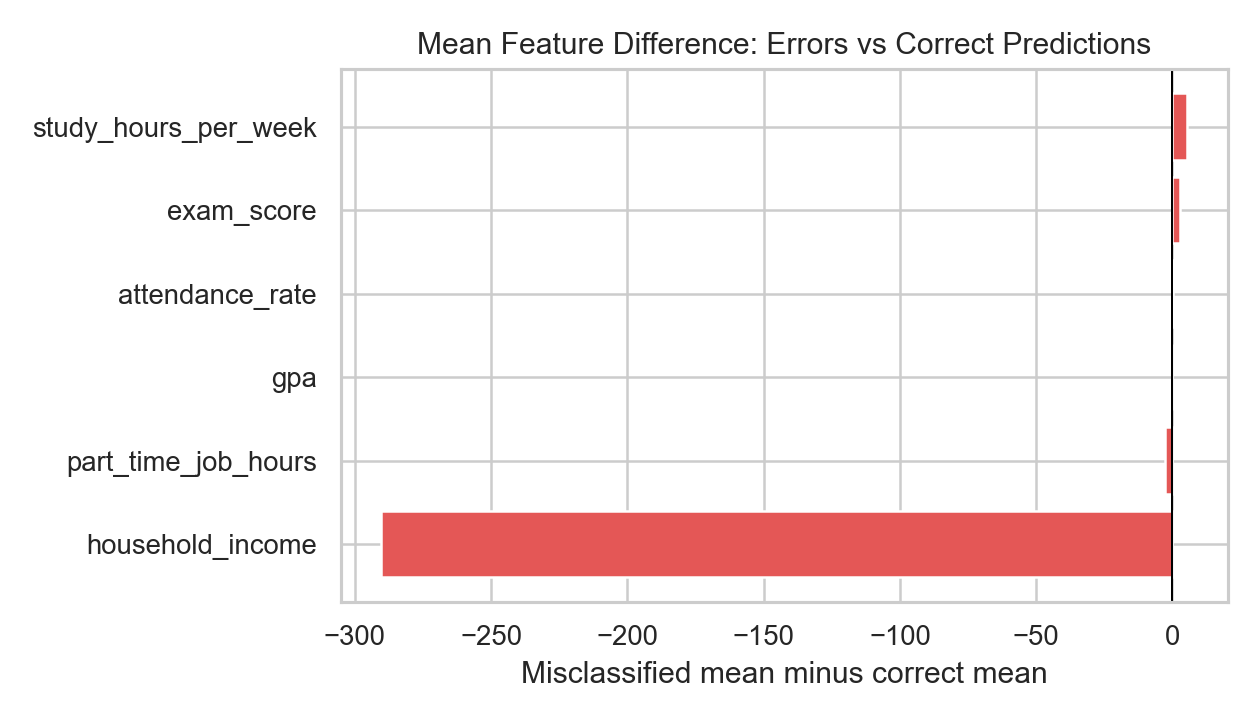
\includegraphics[width=0.82\linewidth]{figures/error_feature_difference.png}
\caption{Mean feature difference between errors and correct predictions.}
\end{figure}

The error cases tend to be borderline cases where some academic signals support scholarship status while other signals are weaker. This is a reasonable limitation for a linear model. The model is reliable when the evidence is strong, but it can be conservative when the signals are mixed.

In a scholarship setting, this trade-off matters. A false negative means that a student who should receive scholarship support is missed. The final recommendation therefore notes that the threshold could be lowered if the institution prioritizes recall over precision.

\clearpage

\section{Model Interpretation}

Model interpretation explains which features the model appears to rely on. This report uses two complementary views: Logistic Regression coefficients and permutation importance.

\subsection{Logistic Regression Coefficients}

\begin{table}[H]
\centering
\caption{Largest Logistic Regression coefficients by absolute value.}
\begin{tabular}{lrr}
\toprule
\textbf{Feature} & \textbf{Coefficient} & \textbf{Absolute Coefficient} \\
\midrule
\texttt{academic\_strength} & 4.4458 & 4.4458 \\
\texttt{gpa} & -1.4748 & 1.4748 \\
\texttt{exam\_score} & -1.2102 & 1.2102 \\
\texttt{household\_income} & -0.5979 & 0.5979 \\
\texttt{income\_per\_study\_hour} & 0.5614 & 0.5614 \\
\texttt{study\_hours\_per\_week} & 0.5445 & 0.5445 \\
\texttt{study\_efficiency} & -0.4362 & 0.4362 \\
\texttt{work\_study\_balance} & 0.4129 & 0.4129 \\
\texttt{attendance\_rate} & 0.3254 & 0.3254 \\
\texttt{part\_time\_job\_hours} & -0.2072 & 0.2072 \\
\bottomrule
\end{tabular}
\end{table}

A positive coefficient increases the predicted probability of scholarship. A negative coefficient decreases it. These values describe model behavior after standardization. They should not be interpreted as causal proof.

\clearpage

\subsection{Permutation Importance}

\begin{figure}[H]
\centering
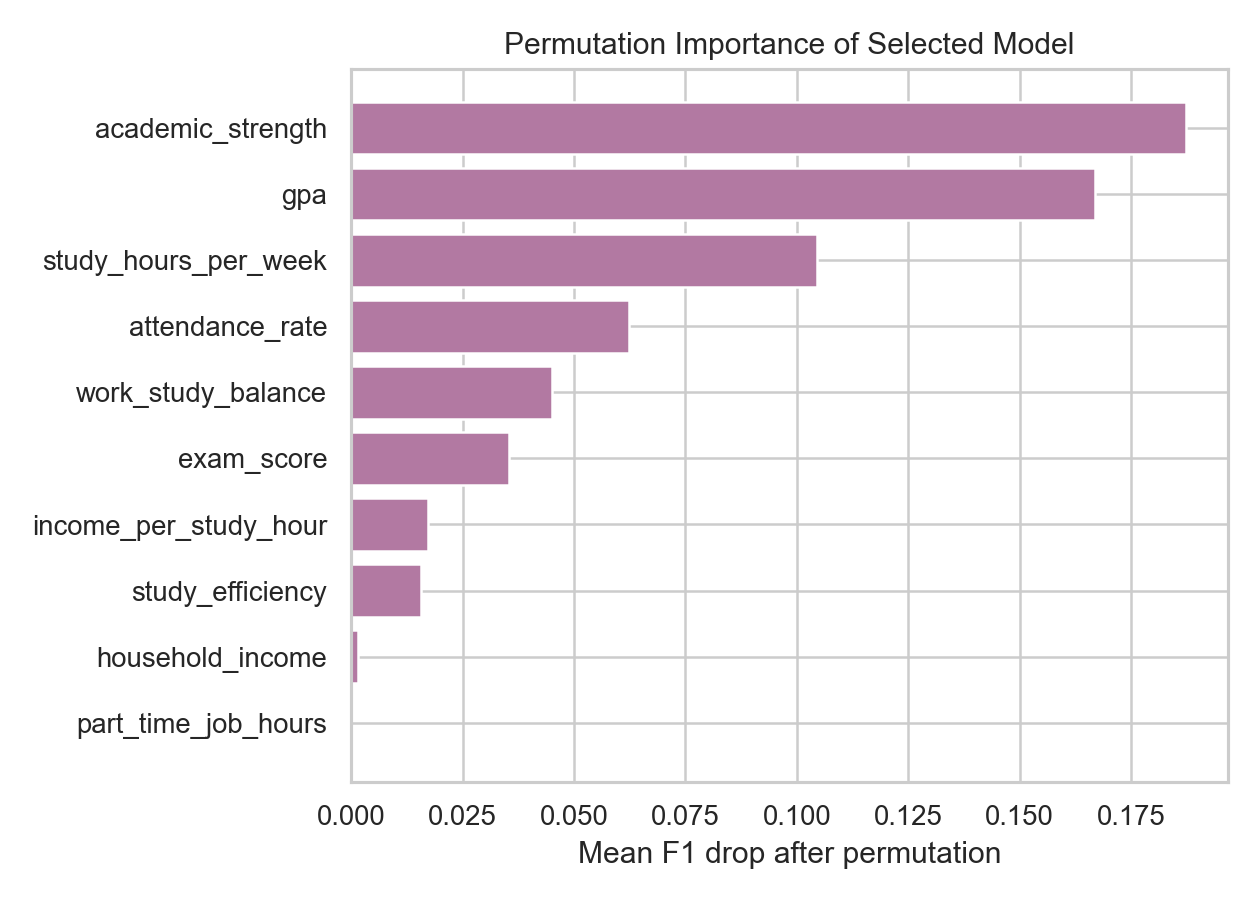
\includegraphics[width=0.82\linewidth]{figures/permutation_importance.png}
\caption{Permutation importance for the selected model.}
\end{figure}

Permutation importance measures how much F1-score drops when one feature is shuffled. A larger drop means the selected model depends more on that feature for prediction. This method is useful because it evaluates the trained model's behavior directly on the development set.

\begin{table}[H]
\centering
\caption{Top permutation importance values.}
\begin{tabular}{lrr}
\toprule
\textbf{Feature} & \textbf{Mean F1 Drop} & \textbf{Standard Deviation} \\
\midrule
\texttt{academic\_strength} & 0.4540 & 0.0612 \\
\texttt{gpa} & 0.0320 & 0.0186 \\
\texttt{exam\_score} & 0.0218 & 0.0163 \\
\texttt{study\_hours\_per\_week} & 0.0170 & 0.0138 \\
\texttt{work\_study\_balance} & 0.0120 & 0.0128 \\
\texttt{attendance\_rate} & 0.0000 & 0.0000 \\
\texttt{household\_income} & 0.0000 & 0.0000 \\
\texttt{part\_time\_job\_hours} & 0.0000 & 0.0000 \\
\bottomrule
\end{tabular}
\end{table}

\clearpage

\section{Final Recommendation and Conclusion}

The recommended model for final submission is Logistic Regression. The main reason is that it provides the strongest balance between performance and interpretability. KNN reached the same F1-score on the development set, but Logistic Regression had a slightly stronger ROC-AUC and is easier to explain with coefficients.

In a scholarship prediction setting, precision and recall have different practical meanings. High precision means the model rarely recommends scholarships for non-recipients. High recall means the model recovers more true scholarship students. The selected model is conservative: it has perfect development precision but lower recall, so the report honestly discusses the remaining false-negative limitation.

Overall, the final project successfully extends the midterm pipeline. It uses the final v2 dataset, adds meaningful engineered features, compares at least three models, includes a controlled tuning strategy, reports required metrics, analyzes errors, interprets model behavior, and generates a valid \texttt{predictions.csv} file.

\subsection{Hidden Test Note}

For local checking, the hidden test file in this workspace contains labels. On this hidden test file, the selected model obtained accuracy 0.8400, precision 0.8333, recall 0.7500, and F1-score 0.7895.

\clearpage

\section{Limitations}

The dataset is synthetic, so the conclusions should not be treated as real educational policy evidence. The model can identify patterns in the provided data, but it cannot prove that any feature causes scholarship decisions.

The prediction file is generated from \texttt{hidden\_test\_data.csv}. Since this file may not include \texttt{part\_time\_job\_hours}, the notebook includes a schema-compatibility step that fills the missing feature with the final training median before producing predictions.

The custom implementations are intended for learning, transparency, and reproducibility. They are not optimized like mature production libraries. However, they satisfy the project constraint and make the algorithmic logic visible in the notebook.

\clearpage

\appendix

\section{Appendix A: Reproducibility Checklist}

\begin{itemize}
    \item The notebook can be run from top to bottom.
    \item The notebook uses relative paths for local and Google Colab usage.
    \item The report is written in English.
    \item The report is compiled from \texttt{main.tex}.
    \item At least three models are trained and compared.
    \item The models are implemented manually without scikit-learn training APIs.
    \item Accuracy, precision, recall, F1-score, ROC-AUC, and confusion matrix are reported.
    \item Error analysis and model interpretation are included.
    \item \texttt{predictions.csv} uses the required \texttt{id,label\_pred} format.
\end{itemize}

\clearpage

\section{Appendix B: Hidden Test Compatibility}

The prediction file is generated from \texttt{hidden\_test\_data.csv}. The workflow is compatible with hidden test files that do not include \texttt{part\_time\_job\_hours}.

If \texttt{part\_time\_job\_hours} is missing, the workflow fills the value with the final training median, which is 13.0. This keeps the prediction pipeline aligned with the final training feature set.

The output format remains:

\begin{verbatim}
id,label_pred
1001,0
1002,1
\end{verbatim}

\clearpage

\section{Appendix C: Submission Checklist}

\begin{longtable}{p{0.65\linewidth}p{0.2\linewidth}}
\caption{Final submission checklist.}\\
\toprule
\textbf{Requirement} & \textbf{Status} \\
\midrule
\endfirsthead
\toprule
\textbf{Requirement} & \textbf{Status} \\
\midrule
\endhead
\texttt{report.pdf} exists & Completed \\
\texttt{main.tex} exists & Completed \\
\texttt{notebook.ipynb} exists & Completed \\
\texttt{predictions.csv} exists & Completed \\
\texttt{README.md} exists & Completed \\
\texttt{requirements.txt} exists & Completed \\
Report follows midterm-style section structure & Completed \\
Report includes final-project improvement section & Completed \\
Notebook avoids scikit-learn imports & Completed \\
Prediction file has \texttt{id,label\_pred} columns & Completed \\
\bottomrule
\end{longtable}

\end{document}

